% \vspace{2ex}
\vspace{-0.3ex}
\section{Experimental Study}
\label{sec-expt}
\vspace{-0.4ex}

\revise{Using standard %database
benchmarks, we conducted four sets of
experiments to evaluate
(1) the overall performance of all benchmark queries with \bdss
computed by our algorithms;
% compared to the traditional tuple-as-a-value model;
(2) the effectiveness of scan-free evaluation;
(3) the quality of \bdss computed by our algorithms vs. the baselines; and
(4) the efficiency of our algorithms.}\looseness = -1


\stitle{Experimental Settings}. We start with the settings.

\eetitle{Benchmarks}. We used two standard benchmarks
\tpch~\cite{tpch} and \imdb~\cite{LeisGMBK015}, including their
data generators (datasets) and built-in queries.
(1) \tpch generates data using {\small TPC-H}
\kw{dbgen}~\cite{tpch}, with 8 relations. It has 22 built-in
parameterized \SQL queries.
(2) \imdb benchmark includes the \imdb relations~\cite{imdbdata}
and \xx real-life \SQL queries~\cite{imdbquery}.
By default, we evaluated the query evaluation performance over
datasets of \xx GB for both benchmarks.

For each relation in the benchmark databases, we assign a random
update frequency in the range of [1, \warn{3}] for testing the
incremental maintenance cost of the generated \bdss. 





%%%%%%%%
\begin{table}[t!]
\vspace*{-1.0em}
\begin{scriptsize}
\begin{center}
{
\setlength{\aboverulesep}{0.0pt}
\setlength{\belowrulesep}{0.0pt}
\setlength{\tabcolsep}{1ex} % for the horizontal padding
\renewcommand{\arraystretch}{1.03}% for the vertical padding
\hspace*{-1ex}\begin{tabular}{c?{0.25mm}c|c|c|c|c|c|c|c|c|c|c}
\toprule
\at{Model} & \bf Q1 &\bf Q2 &\bf Q3 &\bf Q4 &\bf Q5 &\bf Q6 &\bf Q7 &\bf Q8 &\bf Q9 &\bf Q10 &\bf Q11 \\\toprule
% &\bf Q12 &\bf Q13 &\bf Q14 &\bf Q15 &\bf Q16 &\bf Q17 &\bf Q18 &\bf Q19 &\bf Q20 &\bf Q21 &\bf Q22
%\qcs\!(Y/N) & & & & & & & & & & & & & & & & & & & & & & \\\midrule
\at{BaaV} &
\scriptsize  &
\scriptsize  &
\scriptsize  &
\scriptsize  &
\scriptsize  &
\scriptsize  &
\scriptsize  &
\scriptsize  &
\scriptsize  &
\scriptsize  &
\scriptsize   \\\hline
\at{TaaV} &
\scriptsize &
\scriptsize &
\scriptsize &
\scriptsize &
\scriptsize &
\scriptsize &
\scriptsize &
\scriptsize &
\scriptsize &
\scriptsize &
\scriptsize  \\\midrule
\at{Model} &\bf Q12 &\bf Q13 &\bf Q14 &\bf Q15 &\bf Q16 &\bf Q17 &\bf Q18 &\bf Q19 &\bf Q20 &\bf Q21 &\bf Q22 \\\toprule
 \at{BaaV} &
\scriptsize  &
\scriptsize  &
\scriptsize  &
\scriptsize  &
\scriptsize  &
\scriptsize  &
\scriptsize  &
\scriptsize  &
\scriptsize  &
\scriptsize  &
\scriptsize   \\\hline
\at{TaaV} &
\scriptsize &
\scriptsize &
\scriptsize &
\scriptsize &
\scriptsize &
\scriptsize &
\scriptsize &
\scriptsize &
\scriptsize &
\scriptsize &
\scriptsize  \\\midrule
\end{tabular}
}
\end{center}
\end{scriptsize}
\vspace{-0.1em}
\caption{Evaluation time (s: {\normalfont seconds}) of \tpch
  queries %-- {{\normalfont BaaV (with schemas found by \opts) vs. TaaV}}
  \label{expt-tpch-allQ}}
\vspace{-2em}
\end{table}

%%%%%%%%






\eetitle{Parametric queries}.
\warn{We used built-in %parameterized
parameteric \SQL queries of both benchmarks. To evaluate with
larger workloads and the different query complexities, we
further extracted and populated \xx and \xx sub-queries from
\tpch and \imdb built-in queries, with the number \#-\at{join}
of joins varied from \xx to \xx; in total, we had 6 queries for
each \#-\at{join} for each benchmark.}

\vspace{0.6ex}
We assigned a random frequency $w_{Q}$ in the range
of [1, 1000] to each
parametric query $Q$. When testing the total
evaluation time of a query workload, we multiplied the (average)
evaluation time of each query by its frequency and then summed up
over all the queries in the workload; this helps reduce the total
test time by avoiding executing a query for, \eg up to 1000
times, while still providing an accurate overall execution time.
\looseness = -1


\eetitle{Aggregate ranking functions}.
In our experiments, we focused on computing the best \bdss
subject to a storage budget $B$, a setting commonly found in
practice.  \warn{Therefore, we additionally add the size cost
also as a constraint in the ILP programs of \opts
(Section~\ref{sec-select}).}

We tested two aggregate ranking functions
$f(\Q, \kb{\R}) = c_{1}f_{1} + c_{2}f_{2} + c_{3}f_{3}$ (recall
Section~\ref{sec-rank}), where

\vspace{0.6ex}
\bi
\item[(a)] $f^{(a)}(\Q, \kb{\R})$: $c_{1} = \warn{0.9}$,
$c_{2} = \warn{0.1}$ and $c_{3} = 0$.
\item[(b)] $f^{(b)}(\Q, \kb{\R})$: $c_{1} = \warn{0.33}$, $c_{2} =
  \warn{0.33}$ and $c_{3} = \warn{0.34}$.
\ei
Intuitively, $f^{(a)}$ is to compute the \bdss that can make the
largest number of queries scan-free, by maximizing scan-free
evaluability and minimizing the degrees of selected \bdss.
\warn{Here we used a small $c_{2}$ to ensure
that the performance of scan-free query processing over the optimal
\bdss is optimized even the selection algorithm \opts of
Section~\ref{sec-select} takes as input an arbitrary %any arbitrary
universe set $\kb{\A}$.}
Instead, $f^{(b)}$ is to
%prioritize the performance of query evaluation over the \bdss
%while
\warn{take all the criteria with equal importance.}

\warn{Indeed, as will be shown shortly, in practice we found that
the algorithm is quite stable \wrt the coefficients as long as
all the criteria are taken into account in $f(\Q, \kb{\R})$.
It produces similar \baav schemas with variants of $f^{(b)}$
assigned with varying coefficients.}


\eat{%EAT
\vspace{0.6ex}
Observe that the two aggregate ranking functions above represent two
scenarios in practice: if one wants to maximize speedup via
scan-free evaluation, then $f^{(a)}$ is the choice by prioritizing
scan-free evaluability while also minimizing the degrees of the \bdss.
If one additionally considers incremental maintenance cost,
then $f^{(b)}$ fits it the best.
}%EAT



%%%%%%%%%%%%%%
\begin{table}[t!]
\vspace*{-1.0em}
\begin{scriptsize}
\begin{center}
{
\setlength{\aboverulesep}{0.0pt}
\setlength{\belowrulesep}{0.0pt}
\setlength{\tabcolsep}{1ex} % for the horizontal padding
\renewcommand{\arraystretch}{1.03}% for the vertical padding
\hspace*{-1ex}\begin{tabular}{c?{0.25mm}c|c|c|c|c|c|c|c|c|c|c}
\toprule
\at{Model} & \bf Q1 &\bf Q2 &\bf Q3 &\bf Q4 &\bf Q5 &\bf Q6 &\bf Q7 &\bf Q8 &\bf Q9 &\bf Q10 &\bf Q11 \\\toprule
% &\bf Q12 &\bf Q13 &\bf Q14 &\bf Q15 &\bf Q16 &\bf Q17 &\bf Q18 &\bf Q19 &\bf Q20 &\bf Q21 &\bf Q22
%\qcs\!(Y/N) & & & & & & & & & & & & & & & & & & & & & & \\\midrule
\at{BaaV} &
\scriptsize  &
\scriptsize  &
\scriptsize  &
\scriptsize  &
\scriptsize  &
\scriptsize  &
\scriptsize  &
\scriptsize  &
\scriptsize  &
\scriptsize  &
\scriptsize   \\\hline
\at{TaaV} &
\scriptsize &
\scriptsize &
\scriptsize &
\scriptsize &
\scriptsize &
\scriptsize &
\scriptsize &
\scriptsize &
\scriptsize &
\scriptsize &
\scriptsize  \\\midrule
\at{Model} &\bf Q12 &\bf Q13 &\bf Q14 &\bf Q15 &\bf Q16 &\bf Q17 &\bf Q18 &\bf Q19 &\bf Q20 &\bf Q21 &\bf Q22 \\\toprule
 \at{BaaV} &
\scriptsize  &
\scriptsize  &
\scriptsize  &
\scriptsize  &
\scriptsize  &
\scriptsize  &
\scriptsize  &
\scriptsize  &
\scriptsize  &
\scriptsize  &
\scriptsize   \\\hline
\at{TaaV} &
\scriptsize &
\scriptsize &
\scriptsize &
\scriptsize &
\scriptsize &
\scriptsize &
\scriptsize &
\scriptsize &
\scriptsize &
\scriptsize &
\scriptsize  \\\midrule
\end{tabular}
}
\end{center}
\end{scriptsize}
\vspace{-0.1em}
\caption{Evaluation time (s: {\normalfont seconds}) of \imdb
  queries %-- {{\normalfont BaaV (with schemas found by \opts) vs. TaaV}}
  \label{expt-imdb-allQ}}
\vspace{-2em}
\end{table}

%%%%%%%%%%%%%%

\eetitle{Algorithms}. We implemented algorithms \opts
(Section~\ref{sec-select}) and \usc (Section~\ref{sec-cover}).
We used Gurobi~\cite{gurobi} to solve ILP-(I) and ILP-(II) of
\opts.  In particular, when implementing \usc, we lifted the
restriction on the size of $\Sigma$ for procedure \decompose
(see the remark in Section~\ref{sec-cover}). This allows \usc to
generate a larger universe set for \opts; as will be shown
shortly, our approach is still efficient in this case.


\etitle{Baselines}. We also designed two baselines to compare with.

\sstab (1) Algorithm \qcssel that simply returns the collection
of all \qcs of all queries as the schemas, under the
tuple-as-a-value model; that is, it treats each \qcs $W$ as a \bs
$\bschema{\at{id}}{W}$, where $\at{id}$ is an id attribute (or
the candidate key) for $W$.

\sstab (2) Algorithm \uscsel that returns $\kb{\R}$ that consists
of \bss $\kb{R}\bschema{P_{Q}^{R}}{Y_{Q}^{R}}$ for each relation $R$
in each query $Q$ of $\Q$.

\vspace{0.4ex}
Note that by default the \bdss selected by both baselines
are also in the normal form for the query workloads.

In our tests, when the size of the
\bdss $\kb{\R}$ identified by the baselines %algorithms
exceeds the space budget $B$, we remove \bss in $\kb{\R}$ that has
the fewest number of attributes until $\size(\Q, \kb{\R})\leq B$;
if the reduced $\kb{\R}$ is not in the normal form for $\Q$
anymore, we return \texttt{err} and remove them when calculating the
test results.
%the average query evaluation time.





%%%%%%%%%%%%%%%
\begin{figure*}[tb!]
  \vspace*{-2.4ex}
  \begin{subfigure}[b]{1.00\textwidth}
    \setlength{\fboxrule}{0.1pt}
    \centering{\fbox{
\includegraphics[scale=0.33]{./fig/legends-cropped.pdf}}}
    \vspace{0.5ex}
  \end{subfigure}
\begin{subfigure}[b]{1.00\textwidth}
  \centering
        \begin{subfigure}[b]{0.271\textwidth}
			\centering
			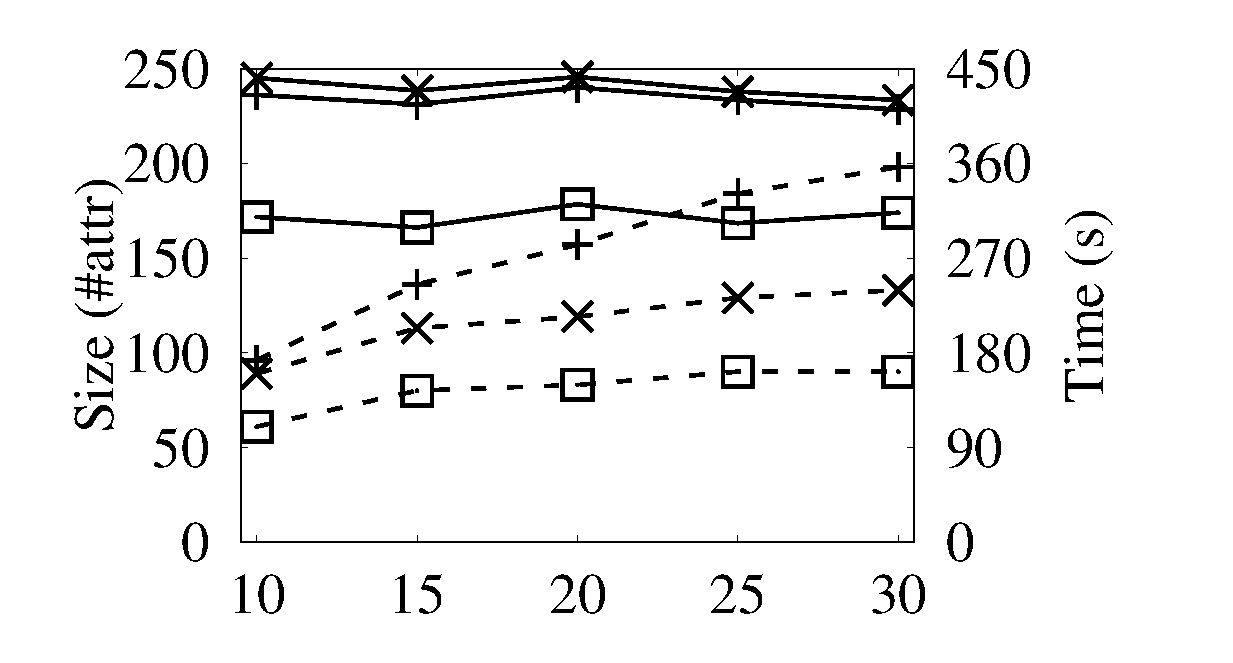
\includegraphics[width=1\textwidth]{fig/vary_q_tpch.eps}
			\begin{center}
				\vspace{-2ex}\caption{\tpch: varying $|\Q|$}
				\label{tpch-1-varyQ}
			\end{center}
			\vspace{-1ex}
        \end{subfigure}
        \hspace{-3ex}
		%
        \begin{subfigure}[b]{0.256\textwidth}
          \centering
          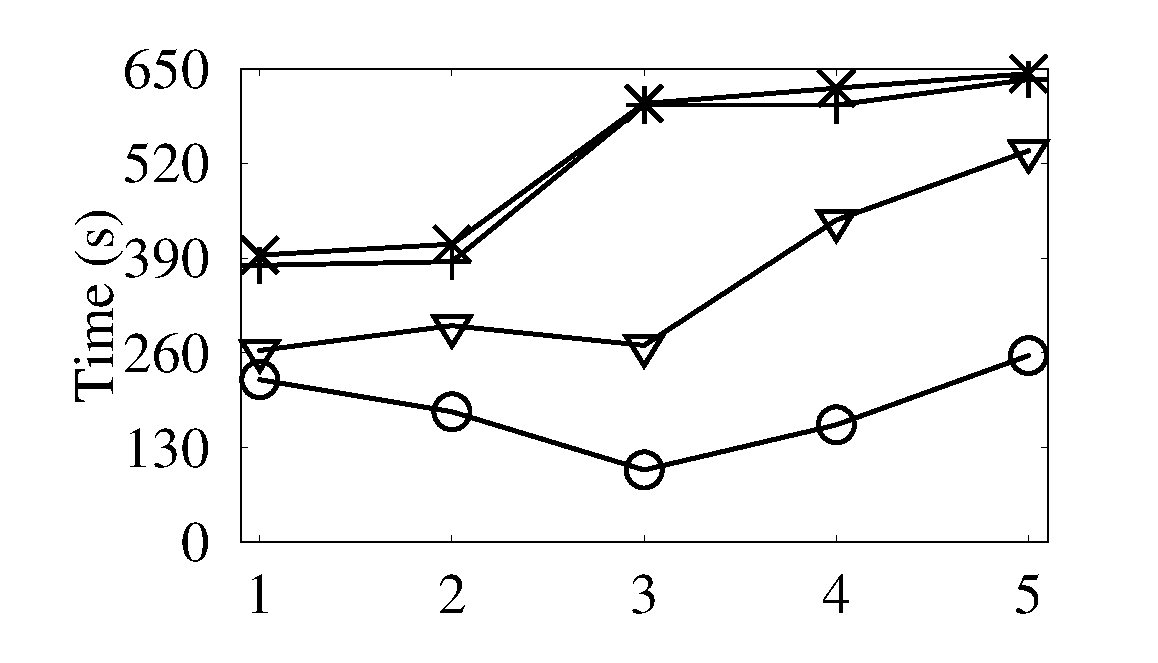
\includegraphics[width=1\textwidth]{fig/vary_j_tpch.eps}
          \begin{center}
            \vspace{-2ex}\caption{\tpch: varying \#-\at{join}}
            \label{tpch-1-vary-join}
          \end{center}
          \vspace{-1ex}
        \end{subfigure}
        \hspace{-2.8ex}
        %
  		\begin{subfigure}[b]{0.256\textwidth}
          \centering
          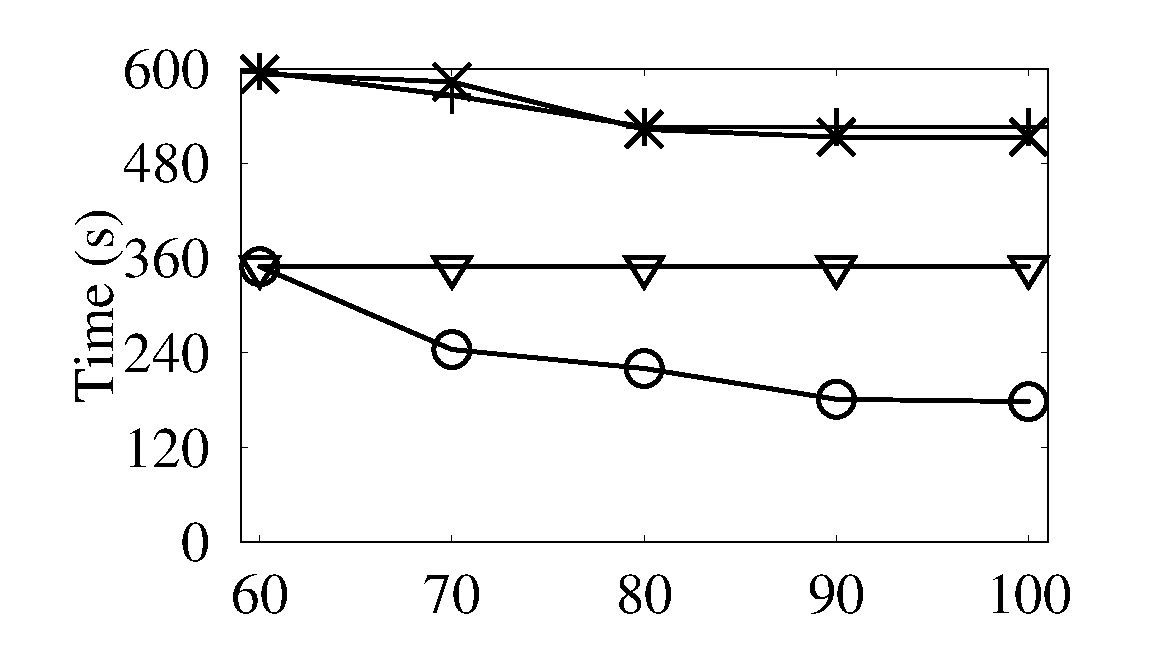
\includegraphics[width=1\textwidth]{fig/vary_b_tpch.eps}
          \begin{center}
            \vspace{-2ex}\caption{\tpch: varying $B$ (\%$B_{\at{max}}$)}
            \label{tpch-1-varyB}
          \end{center}
          \vspace{-1ex}
        \end{subfigure}
        \hspace{-2.8ex}
        %
  		\begin{subfigure}[b]{0.256\textwidth}
          \centering
          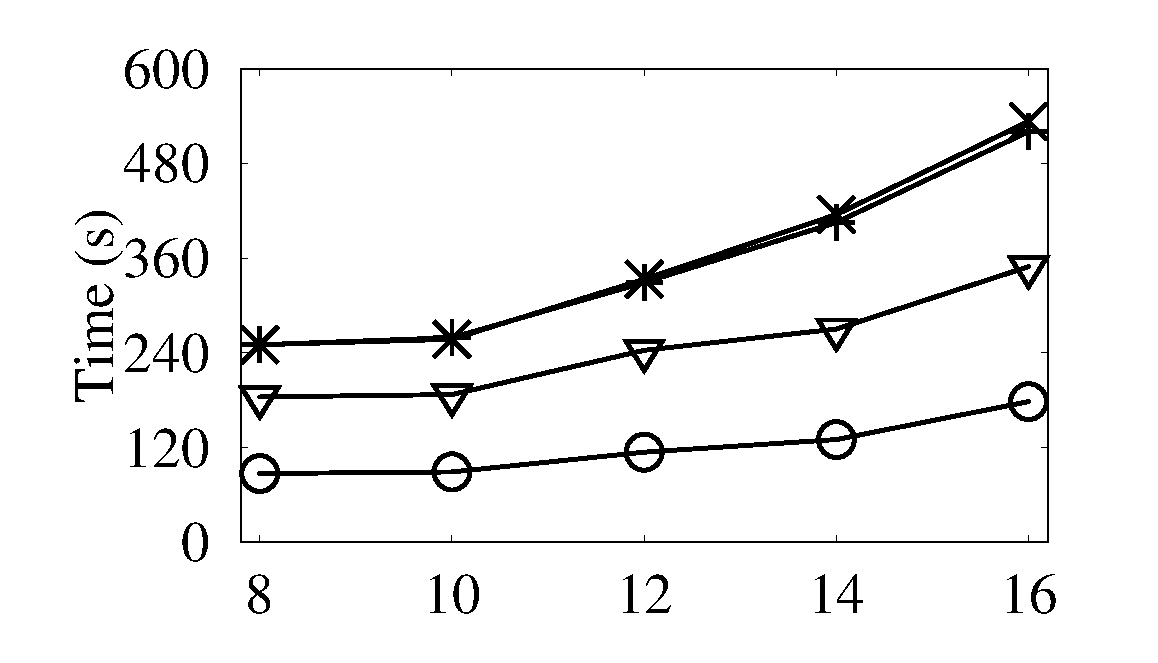
\includegraphics[width=1\textwidth]{fig/vary_d_tpch.eps}
          \begin{center}
            \vspace{-2ex}\caption{\tpch: varying $|\D|$}
            \label{tpch-1-varyD}
          \end{center}
          \vspace{-1ex}
        \end{subfigure}

        \begin{subfigure}[b]{0.271\textwidth}
			\centering
			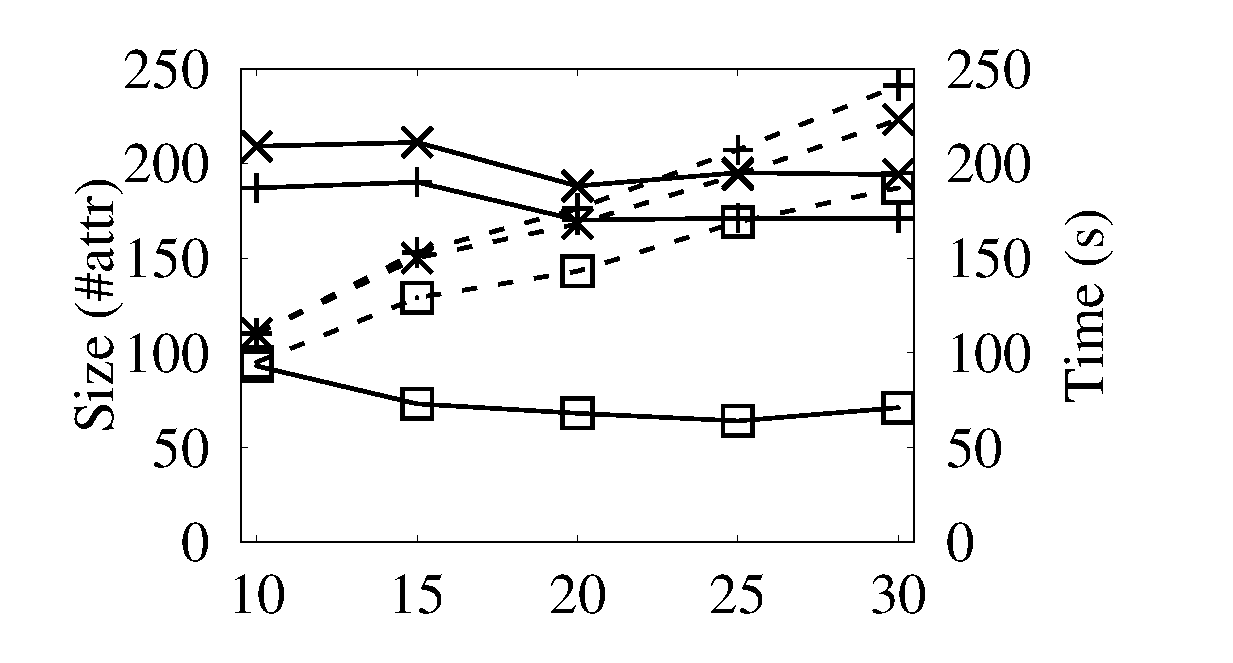
\includegraphics[width=1\textwidth]{fig/vary_q_tpcds.eps}
			\begin{center}
				\vspace{-2ex}\caption{\tpcds: varying $|\Q|$}
				\label{tpcds-1-varyQ}
			\end{center}
			\vspace{-1ex}
        \end{subfigure}
        \hspace{-3ex}
		%
        \begin{subfigure}[b]{0.256\textwidth}
          \centering
          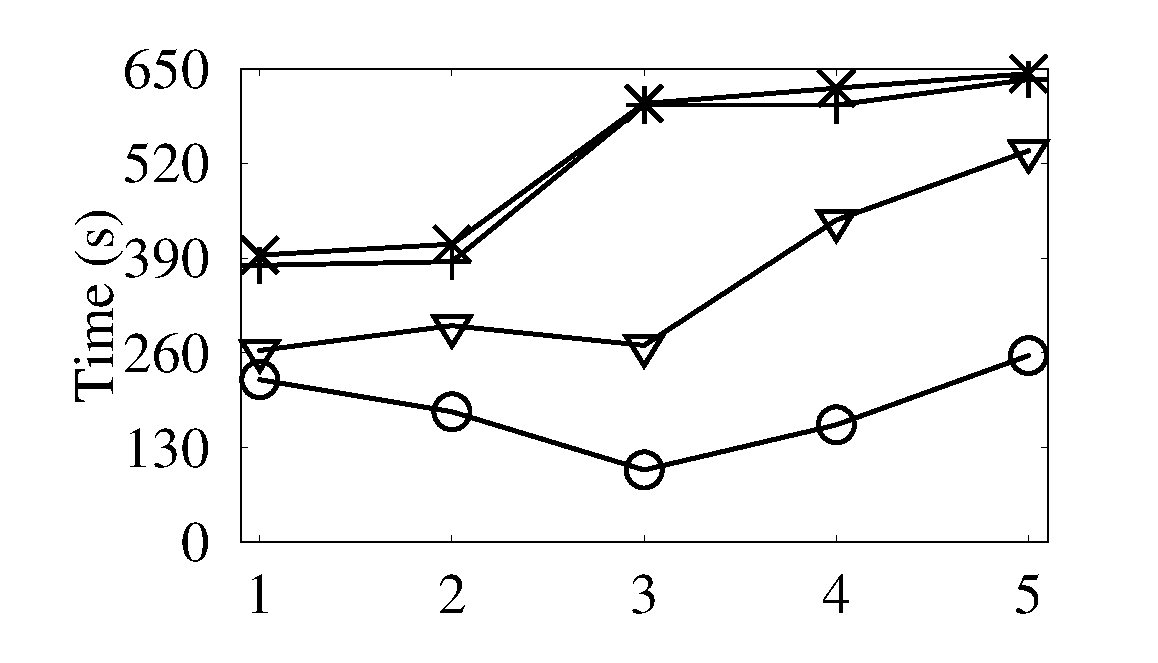
\includegraphics[width=1\textwidth]{fig/vary_j_tpch.eps}
          \begin{center}
            \vspace{-2ex}\caption{\tpcds: varying \#-\at{join}}
            \label{tpcds-1-vary-join}
          \end{center}
          \vspace{-1ex}
        \end{subfigure}
         \hspace{-2.8ex}
        %
  		\begin{subfigure}[b]{0.256\textwidth}
          \centering
          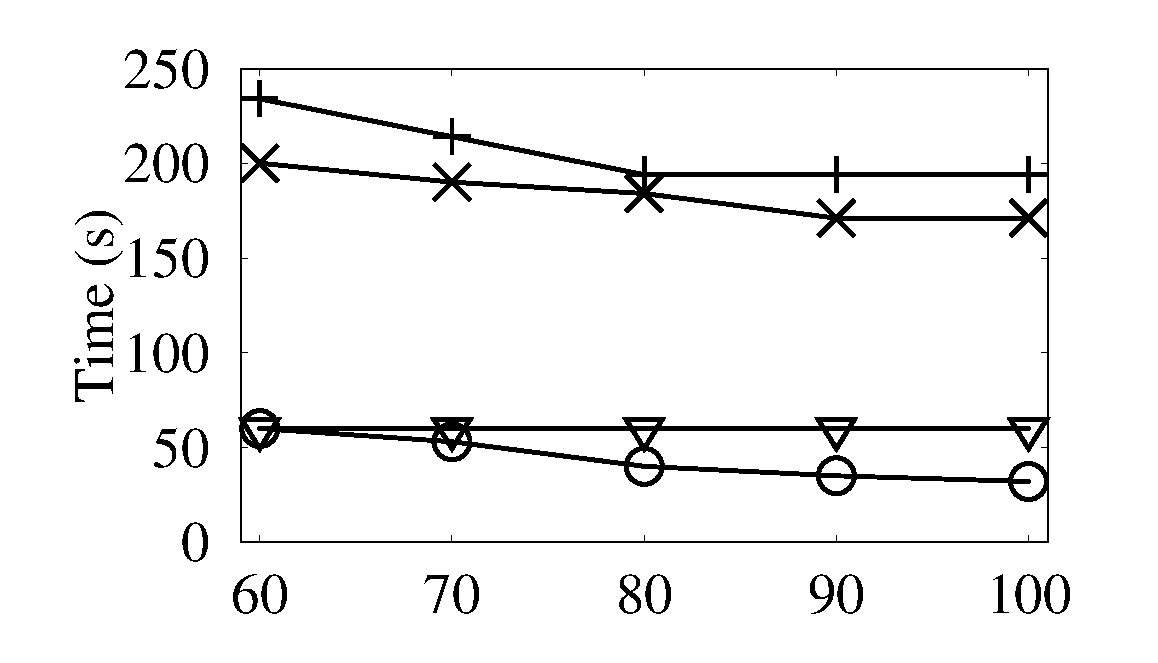
\includegraphics[width=1\textwidth]{fig/vary_b_tpcds.eps}
          \begin{center}
            \vspace{-2ex}\caption{\tpcds: varying $B$ (\%$B_{\at{max}}$)}
            \label{tpcds-1-varyB}
          \end{center}
          \vspace{-1ex}
        \end{subfigure}
         \hspace{-2.8ex}
        %
  		\begin{subfigure}[b]{0.256\textwidth}
          \centering
          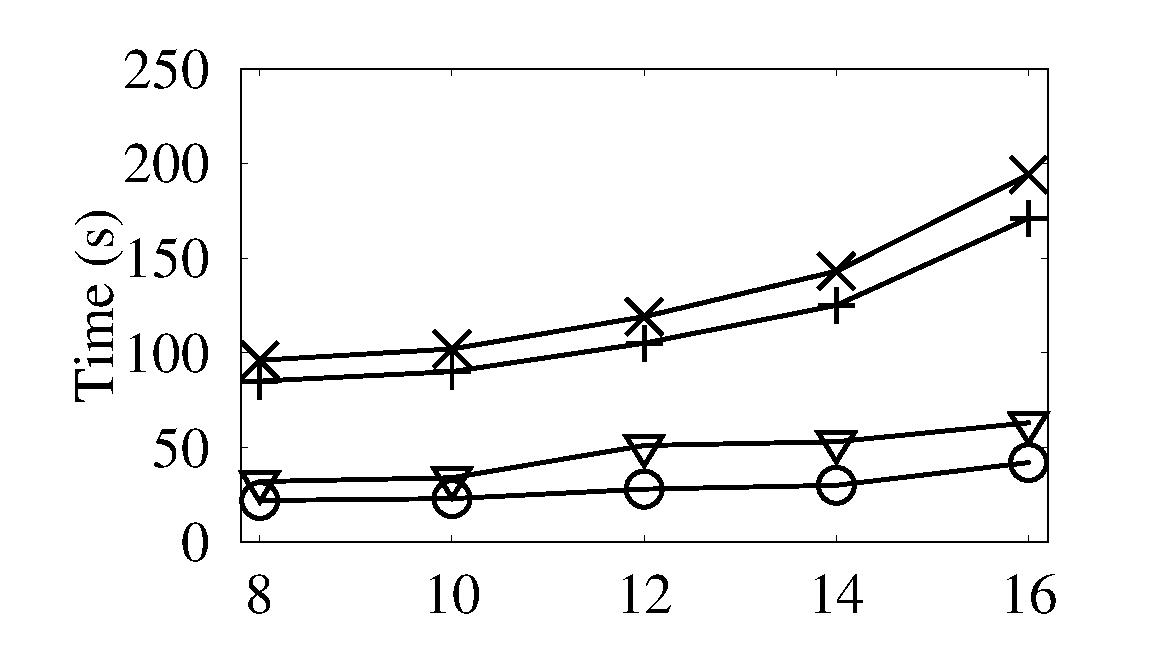
\includegraphics[width=1\textwidth]{fig/vary_d_tpcds.eps}
          \begin{center}
            \vspace{-2ex}
           \caption{\tpcds: varying $|\D|$}
            \label{tpcds-1-varyD}
          \end{center}
          %\vspace{-3.4ex}
        \end{subfigure}
\end{subfigure}
\vspace{-4.0ex}
\caption{Quality evaluation of the computed \bdss ({\bf Exp-3})}
\label{exp-quality}
\vspace{-2.5ex}
\end{figure*}

%%%%%%%%%%%%%%%




\warn{\eetitle{Implementation}.
We used SparkSQL v2.4.0 over Cassandra v3.11.6 as the \kv
system with \SQL evaluation support.
We built the sibling databases according to the computed \bdss by
all the methods, and carried out query evaluation over the
sibling \baav databases using the algorithms of \cite{VLDB19}.
In particular, each \bs $\kb{R}\bschema{X}{Y}$ is
implemented in Cassandra as a table with both $XY$ as the key
such that (a) attributes $X$ must precede $Y$ in the keys and
(b) keys are sorted by $X$. This is a lightweight implementation
of the \baav schemas with Cassandra since it does not require
any modifications to Cassandra.
However, its performance is actually slower than a hack-in
implementation of the \baav model inside Cassandra since
locating the keys for a given $X$-value would incur $O(\log n)$
complexity instead of $O(1)$ asymptotically, assuming there are
$n$ $XY$-values in the relation. This will favor the competitors
when compared to the default SparkSQL-over-Cassandra (tuple-as-a-value model).}


\eetitle{Configuration}.
The experiments were conducted on \warn{a Linux server with \xx CPU,
  \xx GB of memory and \xx GB of HDD disk}.
The server works as both a computing node and a storage node, \ie it works
as a Spark master/slave for the SQL layer (with \xx GB of memory) and also holds a
Cassandra partition for the storage (also with \xx GB of memory).
By default, we set the storage budget $B_{\at{max}}$ of the
\bdss to be 0.7 times of the size of the \imdb database
and 2.5 times for \tpch.
%where size is measured by the number of attributes in our case (other
%more sophisticated size measures can be adopted similarly).
All the tests were run 3 times. The average is reported here.
\looseness = -1






\stitle{Experimental Results}. We next report our findings.

\warn{\stitle{Exp-1: Benchmark tests}. Using default settings, we
first compared the benchmark query performance over \baav
schemas computed by our algorithms and over the conventional
tuple-as-a-value relations. The results are reported in
Table~[\xx]}%\ref{tab-benchmark}.



\warn{\stitle{Exp-2: Scan-free evaluation}.
We then evaluated the effectiveness of scan-free evaluation and
studied the impact of degrees on scan-free queries.}






\stitle{Exp-3: Quality of \bdss}.
We evaluated the quality of the \bdss found by each method in %under
all settings. 


\eetitle{(1) Varying $|\Q|$}. We first compared the minimum
normalized \bdss that can be computed by our method
% with rank functions $f^{(a)}$ and $f^{(b)}$,
and baselines \qcssel and \uscsel.
More specifically, 
let $\Q$ consist of all parametric queries for each benchmark;
we varied the size $|\Q|$ of $\Q$ by randomly sampling queries
from $\Q$ such that $|\Q|$ varies from \warn{10} to \warn{30} for both \tpch and \tpcds. For each $\Q$, we compare the quality of
the minimum \bds $\kb{\R}$ found by each method such that
$\kb{\R}$ is in the normal form for $\Q$ (for our method, we
only need to keep $f_{3}$ in the objective function of \opts,
\ie $c_{i} = 0$ for $i\ak\in\ak \{1,\ak 2,\ak 4\}$).
%(b) $\Q$ is scan-free over $\kb{\R}$.
We assess the quality of such \bdss by (a) their sizes and (b) the
query evaluation time over them.

\sstab (a) As shown by the left $y$-axis of Figures
\ref{tpch-1-varyQ} and \ref{tpcds-1-varyQ}, 
among all methods, our method (shown as \opts)
%with rank function $f^{(b)}$
generates the minimum \bdss that are in the normal
form,
%for the queries,
in all cases. For example, the size of the
minimum normalized \bds computed by \warn{\uscsel} is
\warn{1.57} and \warn{1.15} times larger than our method
%with rank function $f^{(b)}$
when $|\Q| = \warn{10}$ for \tpch
and \tpcds, respectively; it increases to \warn{2.20} and \warn{1.28} times when
$|\Q| = \warn{30}$.
%The minimum normalized \bds computed by our method
%with $f^{{(a)}}$  is slightly larger than our
%method with $f^{(b)}$, but is still on average \xx times smaller
%than those computed by \uscsel.
The results for \qcssel are similar. %to that of \uscsel. 


\sstab (b) For each query $Q$, we define the speedup by method
$A$ over method $B$ as the ratio of the evaluation time of $Q$
on the minimum normalized \bds computed by method $A$ over that
by method $B$; naturally, the average speedup of $\Q$ by method
$A$ over method $B$ is the average of the speedups of queries in
$\Q$ by $A$ over $B$.
As shown by the right $y$-axis of Figures \ref{tpch-1-varyQ} and \ref{tpcds-1-varyQ},
when $|\Q|$ varies from \warn{10} to \warn{30} for
\tpcds, the average speedup by our method
%with rank function $f^{(a)}$
\warn{is \warn{6.31} (resp.~\warn{4.00}) times over algorithm \qcssel
  (resp.~\uscsel) on average, up
to \warn{7.68} (resp. \warn{5.05}) times.}
The results over \tpch are similar.

\vspace{1ex}
These show that our method can find normalized \bdss that are of
smaller size than those found by the baselines (\eg on average \warn{1.43}
times smaller) and %but
provide even faster query evaluation
performance (\eg on average \warn{3.81} times faster).






\eetitle{(2) Varying query complexity (\#-\at{join})}.
We then evaluated the ability of all methods to process complex
queries, \ie queries with varying number of %many
joins. We
classified queries $\Q$ of each benchmark into 5 sub-workloads
$\Q_{i}\ak (i\ak\in\ak [1,\ak 5])$, 
where $\Q_{i}$ consists of all parametric queries in $\Q$ that have exactly $i$
joins. We set the storage budget $B$ to $B_{\at{max}}$ and tested the average
speedup for each sub-workloads in the same ways as in EXP-1(1b)
above. In particular, when a \bds is not in the normal form of a
query $Q$, we evaluate $Q$ directly on the original database and
use the evaluation time to calculate the speedup for $Q$.
For our method, we tested it with both rank functions $f^{(a)}$
and $f^{(b)}$.
\looseness = -1

\vspace{0.6ex}
The results for \tpch and \tpcds are shown in
Figures~\ref{tpch-1-vary-join} and \ref{tpcds-1-vary-join},
respectively. The results tell us the following. 

\sstab (a) Our method works at its best with rank
function $f^{(a)}$ in %terms of the
query performance.
The average query speedup achieved by our method
with rank function $f^{(a)}$ over %it
with
$f^{(b)}$ is \warn{2.14} and \warn{2.52} times on average for \tpch and \tpcds,
respectively, up to \warn{4.71} and \warn{27.96} times.
Moreover, no matter with which rank function, it always
provides \bdss better than both \qcssel and \uscsel do.
For example, with $f^{(a)}$ it is on average \warn{5.57} and \warn{11.36}
times better than \qcssel over \tpch and \tpcds, respectively,
up to \warn{34.76} and \warn{71.40} times; for $f^{(b)}$ it is \warn{3.10} and
\warn{6.38} times on average, respectively, up to \warn{19.92} and \warn{35.97} times.
%the numbers for $f^{(b)}$ are \xx and
%\xx times on average, up to \xx and \xx times.
\looseness = -1

\sstab (b) Our method with both rank functions $f^{(a)}$ and
$f^{(b)}$ are able to handle complex queries much better than
the baselines, and the gap gets bigger when the number
of joins (\#-\at{join}) increases.
For instance, when \#-\at{join} increases from \warn{1} to \warn{5} over
\tpcds, the average speedup by our method with $f^{(a)}$ over
\qcssel increases from \warn{15.26} to \warn{17.05} times; the gap is \warn{1.63} and \warn{16.91}
times over \uscsel; the results are similar for \tpch.


\sstab (c) However, this comes with a price: the maintenance cost
of the \bdss computed by our method with $f^{(a)}$ is \warn{4.04} times
larger than the cost with $f^{(b)}$ on average,
where the cost is measured by $\update(\Q, \kb{\R})$ (recall Section~\ref{sec-rank}). 


\eetitle{(3) Varying space budget $B$}. We next evaluated the
quality of \bdss computed by our method under varying storage
budget $B$. Varying $B$ from \warn{60}\%$B_{\at{max}}$ to
$B_{\at{max}}$, we compared the average evaluation time per query
of all methods. We used all parametric queries for each
benchmark.
% When the size of the
% \bdss $\kb{\R}$ identified by the baseline algorithms
% exceeds the space budget $B$, we remove \bss in $\kb{\R}$ that has
% the fewest number of attributes until $\size(\Q, \kb{\R})\leq B$;
% if the reduced $\kb{\R}$ is not in the normal form for $\Q$
% anymore, we return \texttt{err} and remove them when calculating
% the average query evaluation time for the baselines. 
The results for \tpch and \tpcds are reported in
Figures~\ref{tpch-1-varyB} and \ref{tpcds-1-varyB}.
We observed the following.

\sstab (a) Consistent with Exp-1(1a), our method with both
rank functions is able to identify \bdss that
are in the normal form under small space budget $B$,
while the baselines cannot.

\sstab (b) Queries are answered more efficiently on \bdss
computed by our method than over those found by the baselines,
for both rank functions.
Moreover, the gaps become even larger when $B$ is
smaller. For example, the average speedup by our method with
rank function $f^{(a)}$ over algorithm \qcssel is on average \warn{4.44}
times, and up to \warn{34.76} times over \tpch; the speedup is %speedups are
\warn{8.56} times
on average over \tpcds, up to \warn{71.40} times.
\looseness = -1

\sstab (c) Consistent with other experiments reported
above, our method works \warn{better with rank
function $f^{(a)}$ than with $f^{(b)}$}
in terms of query evaluation performance.
Moreover, the larger $B$ becomes, the bigger the gap is. 
For example, when $B$ increases from \warn{60}\%$B_{\at{max}}$ to
$B_{\at{max}}$, the speedup by
our method with $f^{(a)}$ over with $f^{(b)}$ \warn{increases} from \warn{1.05}
to \warn{2.14} times over \tpch. 



\eetitle{(4) Varying dataset size}.
We finally evaluated the quality of the \bdss by testing them
with datasets of different sizes. We
varied the size of the datasets $D$ from \warn{8}GB to \warn{16}GB and
compared the query evaluation time in the same setting
of EXP-1(3) above,
except that  $B$ is fixed to $B_{\at{max}}$ instead.
The results over \tpch and \tpcds are reported in
Figures~\ref{tpch-1-varyD} and \ref{tpcds-1-varyD}, respectively.
Consistent with other experiments, our method with $f^{(a)}$ computes the best
\bdss in terms of query evaluation performance, and its gap over
others increases when the dataset grows bigger, \eg
from \warn{5.97} to \warn{7.13} times when the \tpcds dataset increases from \warn{8} GB to \warn{16} GB.


%%%%%%%%%%%%%%%%% EXP-2
\begin{table}
  \begin{center}
    \begin{footnotesize}
      \caption{Efficiency of our method (\opts and \usc) ({\bf
          Exp-2}) (\textnormal{\footnotesize $\kb{\R}$ is the \bds returned by
          \opts; $\kb{\A}$ is the universe set computed by \usc;
          the evaluation time includes that of both \opts and \usc}) \label{exp-2}}
      \setlength{\aboverulesep}{0.1pt}
      \setlength{\belowrulesep}{0.5pt}
      \setlength{\tabcolsep}{2ex} % for the horizontal padding
      \renewcommand{\arraystretch}{1.1}% for the vertical padding
      %\vspace{-0.7ex}
      \hspace*{-0.8ex}\begin{tabu}{l|[0.30mm]l|[0.15mm]l|[0.15mm]l|[0.30mm]l|[0.15mm]l|[0.15mm]l}
        \toprule
        \multirow{2}{*}{\bf $f(\Q, \kb{\R})$} & \multicolumn{3}{c|[0.30mm]}{\textbf{TPC-H}} & \multicolumn{3}{c}{\textbf{TPC-DS}} \\\cline{2-7}
        & \multicolumn{1}{c|}{$|\kb{\R}|$} & \multicolumn{1}{c|}{$|\kb{\A}|$} & \multicolumn{1}{c|[0.30mm]}{time} & \multicolumn{1}{c|}{$|\kb{\R}|$} & \multicolumn{1}{c|}{$|\kb{\A}|$}   & \multicolumn{1}{c}{time}  \\\midrule
        $f^{(a)}$ &  149& 272&  0.42& 271& 376 & 0.27\\\hline
        $f^{(b)}$ &  91& 272&  0.39& 187& 376 & 0.23\\\bottomrule
      \end{tabu}
    \end{footnotesize}
  \end{center}
  \vspace{-3.4ex}
\end{table}
%%%%%%%%%%%%%%%%% 

%\vspace{0.36ex}
\stitle{Exp-4: Efficiency}.
We also evaluated the efficiency of our method.
We used the same setting as EXP-1(4) and tested
%We used all queries for both benchmarks and tested
(a) the size $|\kb{\A}|$ of the universe set $\kb{\A}$ computed by \usc;
(b) the size $|\kb{\R}|$ of the final \bds $\kb{\R}$ returned by \opts; and
(c) the total time taken by our method (\ie \opts and \usc).
%for computing $\kb{\R}$.
The results of our algorithms
%with both rank functions
are reported in Table~\ref{exp-2}. It shows that our algorithms are
efficient, and the universe set is of moderate size while being
able to cover the optimal \bdss. 


\stitle{Summary}. From the experimental study we find the following.
  (1)  The \bdss computed by our algorithms are effective.
  Over the computed  \bdss with SparkSQL-over-Cassandra,
  on average \tpch and \tpcds queries can be made \warn{4.28} and \warn{7.01}
 times faster than over the \bdss computed by the baselines,
 respectively.
 %and \xx and \xx times faster than executing directly
 %over relations stored under
 %the conventional tuple-as-a-value model in Cassandra.
 (2) Moreover, the gap increases when the queries are more
 complex (\ie with more joins) or the datasets grow bigger.
 (3) \warn{Our algorithms are efficient: they finish in
 0.42 and 0.27 seconds for \tpch and \tpcds, respectively.}


\eat{%EAT
  \begin{figure*}[tb!]
%\vspace{-1.7ex}
\begin{subfigure}[b]{1.00\textwidth}
  \centering
        \begin{subfigure}[b]{0.245\textwidth}
			\centering
			
\includegraphics[width=1\textwidth]{fig/a.eps}
			\begin{center}
				\vspace{-2ex}\caption{\tpch: varying $|\Q|$}
				\label{tpch-1-varyQ} 
			\end{center}
			\vspace{-1ex}
        \end{subfigure}
        %\hspace{-2.2ex}
		%
        \begin{subfigure}[b]{0.245\textwidth}
          \centering
          
\includegraphics[width=1\textwidth]{fig/a.eps}
          \begin{center}
            \vspace{-2ex}\caption{\tpch: varying \#-\at{join}}
            \label{tpch-1-vary-join} 
          \end{center}
          \vspace{-1ex}
        \end{subfigure}
        % \hspace{-2.2ex}
        %
  		\begin{subfigure}[b]{0.245\textwidth}
          \centering
          
\includegraphics[width=1\textwidth]{fig/a.eps}
          \begin{center}
            \vspace{-2ex}\caption{\tpch: varying $B$}
            \label{tpch-1-varyB} 
          \end{center}
          \vspace{-1ex}
        \end{subfigure}
        % \hspace{-2.2ex}
        % 
  		\begin{subfigure}[b]{0.245\textwidth}
          \centering
          
\includegraphics[width=1\textwidth]{fig/a.eps}
          \begin{center}
            \vspace{-2ex}\caption{\tpch: varying $|\D|$}
            \label{tpch-1-varyD} 
          \end{center}
          \vspace{-1ex}
        \end{subfigure}

        \begin{subfigure}[b]{0.245\textwidth}
			\centering
			
\includegraphics[width=1\textwidth]{fig/a.eps}
			\begin{center}
				\vspace{-2ex}\caption{\tpcds: varying $|\Q|$}
				\label{tpcds-1-varyQ} 
			\end{center}
			\vspace{-1ex}
        \end{subfigure}
        %\hspace{-2.2ex}
		%
        \begin{subfigure}[b]{0.245\textwidth}
          \centering
          
\includegraphics[width=1\textwidth]{fig/a.eps}
          \begin{center}
            \vspace{-2ex}\caption{\tpcds: varying \#-\at{join}}
            \label{tpcds-1-vary-join} 
          \end{center}
          \vspace{-1ex}
        \end{subfigure}
        % \hspace{-2.2ex}
        %
  		\begin{subfigure}[b]{0.245\textwidth}
          \centering
          
\includegraphics[width=1\textwidth]{fig/a.eps}
          \begin{center}
            \vspace{-2ex}\caption{\tpcds: varying $B$}
            \label{tpcds-1-varyB} 
          \end{center}
          \vspace{-1ex}
        \end{subfigure}
        % \hspace{-2.2ex}
        % 
  		\begin{subfigure}[b]{0.245\textwidth}
          \centering
          
\includegraphics[width=1\textwidth]{fig/a.eps}
          \begin{center}
            \vspace{-2ex}\caption{\tpcds: varying $|\D|$}
            \label{tpcds-1-varyD} 
          \end{center}
          \vspace{-1ex}
        \end{subfigure}
      \end{subfigure}
\caption{Quality evaluation of the computed \bdss ({\bf Exp-1})}
\label{exp-quality}
\end{figure*}
    

\section{Experimental Study}
\label{sec-expt}

Using standard benchmarks, we conducted two sets of experiments to evaluate
(1) the quality of \bdss computed by our algorithms; and
(2) the efficiency of our algorithms.


\stitle{Experimental Settings}. We start with the settings.

\eetitle{Benchmarks}. We used two standard benchmarks
\tpch~\cite{tpch} and \tpcds~\cite{tpcds}, including their 
data generators and built-in parametric queries.
(1) \tpch generates data using {\small TPC-H}
\kw{dbgen}~\cite{tpch}, with 8 relations. It has 22 built-in
parameterized \SQL queries.
(2) \tpcds generates data using {\small
TPC-DS} \kw{dbgen}~\cite{tpcds}, with 24 relations. It has 99
built-in parametric \SQL queries.
By default, we evaluated the query evaluation performance over
datasets of 16GB for both benchmarks. 

For each relation in the benchmark databases, we assign a random
update frequency in the range of [1, 10] for testing the
incremental maintenance cost of the generated \bdss. 


\eetitle{Parametric queries}. We used all built-in
parameterized queries of both benchmarks. When a query is not
\SPC, we used its \SPC sub-queries instead. After this, we have
\xx and \xx\ parametric \SPC\ \tpch and \tpcds queries, respectively (only
16 \tpch queries contain sensible \SPC sub-queries with
selections); all of them are K-FK join only queries. To evaluate
with larger workloads and varying query complexities, we also
generated \xx and \xx parametric \SPC queries for \tpch and \tpcds,
respectively, with the number of joins varying from \warn{0} to
\warn{3}.


We assign a random frequency $w_{Q}$ in the range of [1, 1000] to each
parametric query $Q$. In our tests, when evaluate the total
evaluation time of a query workload, we multiply the (average)
evaluation time of each query by its frequency and then sum up
over all the queries in the workload; this helps reduce the total
test time by avoiding executing a query for, \eg up to 1000
times, while still providing an accurate overall execution time.
\looseness = -1


\eetitle{Aggregate ranking functions}.
In our test, we focus on computing the best \bdss subject to a
storage budget $B$. Therefore, we treat the space cost (\ie
measure (3)) as a constraint in the ILP programs of algorithm
\opts (Section~\ref{sec-select}). For convenience, we used the
number of total attributes to measure the space cost of the
\bdss; note that this is not a restriction of our approach as the
measures and algorithms treat the estimated space cost as input
and hence support any more sophisticated space cost estimation
for measure (3) as an input.


We used four aggregate ranking functions $f(\Q, \kb{\R}) = c_{1}f_{1} +
c_{2}f_{2} + c_{3}f_{3} + c_{4}f_{4}$ (recall
Section~\ref{sec-rank}), where 
\bi
\item[(a)] $f^{(a)}(\Q, \kb{\R})$: $c_{1} = 1$, $c_{i} = 0(i\in [2,4])$.
\item[(b)] $f^{(b)}(\Q, \kb{\R})$: $c_{1} = 0.9999$ and $c_{2} = 0.0001$. 
\item[(c)] $f^{(c)}(\Q, \kb{\R})$: $c_{1} = 0.01$, $c_{2} = 0.0001$ and $c_{4}
  = 0.9899$. 
\item[(d)] $f^{(d)}(\Q, \kb{\R})$: $c_{1} = 0.9899$, $c_{2} =
  0.0001$ and $c_{4} = 0.01$.
\ei
Intuitively, $f^{(a)}$ is to compute the \bdss that can make the
largest number of queries bounded, by using measure (1) only; 
$f^{(b)}$ is to enhance measure (1) with measure (2), to further
improve the performance of queries over the optimal \bdss;
$f^{(c)}$ is to give priority to the maintenance cost, \ie
measure (4); and $f^{(d)}$ is to give priority to the performance
of queries over the \bdss while also taking into account the
incremental maintenance with a lower priority.

Observe that the four aggregate ranking functions above models
four scenarios in practice: if one concerns the number of queries
with the scan-free evaluability property, then $f^{(a)}$ is the
one to go; if one wants to additionally maximize the performance
gains, then $f^{(b)}$ gives more control on the \bdss; if one
additionally considers incremental maintenance cost but is less
important than query evaluation performance, then $f^{(d)}$ fits
best; if one cares incremental performance most, then $f^{(c)}$
captures the objective best with all three measures taken
together.
\looseness = -1


\eetitle{Algorithms}. We implemented our algorithms \opts
(Section~\ref{sec-select}) and \usc (Section~\ref{sec-cover}). We
used Gurobi~\cite{gurobi} to solve ILP-(I) and ILP-(II) of \opts.
In particular, when implementing \usc, we lifted the restriction
on the size of $\Sigma$ of procedure \decompose (see the remark
at the end of Section~\ref{sec-cover}). This allows \usc to
generate a larger universe set for \opts; as will be shown
shortly, the our approach is still efficient. 

\vspace{0.7ex}
We also designed two baselines.

\vspace{-0.4ex}
\etitle{(1) Algorithm \qcssel} that simply returns the collection
of all \qcs of all queries as the schemas, under the
tuple-as-a-value model; that is, it treats each \qcs $W$ as a \bs
$\bschema{\at{id}}{W}$, where $\at{id}$ is an id attribute (or
the candidate key) for $W$.

\vspace{-0.4ex}
\etitle{(2) Algorithm \uscsel} that returns $\kb{\R}$ for
consisting of $\kb{R}_{Q}^{1}$ generated in Step (1)
of \usc (Section~\ref{sec-cover}) for each query $Q$.

\vspace{0.4ex}
Note that, the \bdss selected by both baselines are in the normal
form for the query workload. 

\eetitle{Configuration}.
The experiments were conducted on a cluster of \warn{4} Amazon
EC2 \warn{m4.2xlarge} instances, with \warn{32}GB of memory, \warn{8}
vCPUs and \warn{500}GB of NVMe SSD for each instance.
We used \warn{SparkSQL v\xx over Cassandra v\xx} as the \kv
system with \SQL evaluation support.
We built the sibling databases according to the computed \bdss by
all the methods, and carried out query evaluation over the
sibling \baav databases by following \cite{VLDB19}. 
Each EC2 instance works as both a computing node and a storage node, \ie it works
as a Spark master/slave for the SQL layer and also holds a
Cassandra partition for the storage (with a dedicated Spark
master node).
% We also used one additional instance as the Spark master.
All the tests were run 3 times. The average is reported here.


\stitle{Experimental Results}. We next report our findings.

\stitle{Exp-1: Quality of \bdss}.
We evaluated the quality of the \bdss found by every method under
every setting. 

\eetitle{(1) Varying $|\Q|$}. We first assess the quality of the
computed \bdss by evaluating the average query evaluation time
per each instantiated query over query workloads of varying sizes.
More specifically, let $\Q$ consists of all parametric queries
for each benchmark; we varied the size $|\Q|$ of $\Q$ by randomly
sampling queries from $\Q$ such that $|\Q|$ varies from \xx to
\xx for \tpch and \xx to \xx for \tpcds. We set the space budget
$B$ to the total number $B_{\at{max}}$ of attributes in the database schema of
each benchmark, \ie the generated \bdss are no larger than the
original database schemas. For both \tpch and \tpcds, we generate
database instances of size \xx GB. We instantiated each
parametric query by randomly drawing values from the database
instances for the parameters. To save time, for each parametric
query $Q$, we evaluated five queries instantiated from $Q$ and
used their average evaluation time as the evaluation time $t_{Q}$
for $Q$. For a workload $\Q$, we calculated the average evaluated
time per query as $\sum_{Q\in \Q} w_{Q}*t_{Q}/\sum_{Q\in \Q}w_{Q}$.

The results for \tpch and \tpcds are reported in
Fig.~\ref{tpch-1-varyQ} and \ref{tpcds-1-varyQ}, respectively.
We found the following. 

\sstab (a) All \bdss generated by all methods are in the normal
form and hence all queries can be answered. 

\sstab (b) Our method with ranking function $f^{(b)}$
consistently generated \bdss over which queries are answered the
most efficiently. This followed by our method with ranking
function $f^{(d)}$. Baseline \qcssel is the worst.
For example, 


\sstab (c) The larger $|\Q|$ is, the better our method performs
when compared to the baselines. For example, 


\sstab (d) In particular, while ranking function $f^{(c)}$ gives
the large majority of weight (98.99\%) to minimizing incremental
maintenance cost, with out algorithms it still identifies \bdss
that are more efficient then baseline \qcssel while yielding
smaller maintenance cost at the same time. 
For example, 


\eetitle{(2) Varying query complexity (\#-\at{join})}.
We then evaluated the ability of all methods to process complex
queries, \ie queries with many joins. More specifically, we
classified queries of each benchmark workload $\Q$ into 4 sub-workloads
$\Q_{1}$, $\Q_{2}$, $\Q_{3}$ and $\Q_{4}$, where $\Q_{i}$
consists of all parametric queries in $\Q$ that have exactly $i$
joins. We set the space budget $B$ and tested the average
evaluation time per each instantiated query of each sub-workloads
in the same ways as in EXP-1(1) above.

The results for \tpch and \tpcds are shown in
Fig.~\ref{tpch-1-vary-join} and \ref{tpcds-1-vary-join},
respectively. They tell us the following. 

\sstab (a) Our methods deal with complex queries much better than
the baselines and the gap increases when the number of joins
(\#-\at{join}) increases. 
For instance, 

\sstab (b) Our method with ranking function $f^{(b)}$ works at
its best in terms of the average query evaluation time. In
particular, its gaps over our method with ranking functions
$f^{(c)}$ and $f^{(d)}$ becomes larger when \#-at{join} increases.
For instance, 


\sstab (c) However, this comes with a price: the maintenance cost
of the \bdss computed by our method with $f^{(b)}$ is \xx times
larger than it with $f^{(c)}$, where the cost is measured by
$\update(\Q, \kb{\R})$ (recall Section~\ref{sec-rank}). 
For instance, 


\eetitle{(3) Impact of space budget $B$}. We next evaluated the
quality of \bdss computed by our method under varying storage
budget $B$. Varying $B$ from 40\%$B_{\at{max}}$ to
$B_{\at{max}}$, we compared the average evaluation time per query
of all methods. We used all parametric queries for each
benchmark. When the \bdss $\kb{\R}$ identified by the baseline algorithms
exceeds the space budget $B$, we remove \bss in $\kb{\R}$ with
the fewest number of attributes until $\size(\Q, \kb{\R})\leq B$;
if the reduced $\kb{\R}$ is not in the normal form for $\Q$
anymore, we return \texttt{err} and remove them when calculating
the average query evaluation time for the baselines. 
The results for \tpch and \tpcds are given in
Fig.~\ref{tpch-1-varyB} and \ref{tpcds-1-varyB}.
We observed the following.

\sstab (a) Our method with all four ranking functions can
identify \bdss that are in the normal form under small space
budget $B$ when the baselines cannot.
For example, 


\sstab (b) Queries are answered more efficiently on \bdss
computed by our methods than over those find by the baselines,
for all ranking functions.  Moreover, the gaps are even larger
when $B$ is smaller. For example, 


\sstab (c) Consistent with other experiments, our method works
best with ranking function $f^{(b)}$ in terms of the average
query evaluation time. For example, 


\eetitle{(4) Varying dataset size}.
We finally evaluated the quality of the \bdss by testing them
with varied size of datasets. More specifically, we varied the
size of the datasets from 4GB to 16GB and compared the average
query evaluation time following the setting of EXP-1(3) above
with $B$ fixed to $B_{\at{max}}$ instead.
The results for \tpch and \tpcds are reported in
Fig.~\ref{tpch-1-varyD} and \ref{tpcds-1-varyD}, respectively.
They tell us that our method with $f^{(b)}$ computes the best
\bdss in terms of query evaluation performance, and its gap over
others increases when the dataset grow. For example, 


%%%%%%%%%%%%%%%%% EXP-2
\begin{table}
  \begin{center}
    \begin{footnotesize}
      \caption{Efficiency of our method (\opts and \usc) ({\bf
          Exp-2}) (\textnormal{\footnotesize $\kb{\R}$ is the \bds returned by
          \opts; $\kb{\A}$ is the universe set computed by \usc;
          the evaluation time includes that of both \opts and \usc}) \label{exp-2}}
      \setlength{\aboverulesep}{0.1pt}
      \setlength{\belowrulesep}{0.5pt}
      \setlength{\tabcolsep}{1.5ex} % for the horizontal padding
      \renewcommand{\arraystretch}{1.08}% for the vertical padding
      \hspace*{-0.8ex}\begin{tabu}{l|[0.30mm]l|[0.15mm]l|[0.15mm]l|[0.30mm]l|[0.15mm]l|[0.15mm]l}
        \toprule
        \multirow{2}{*}{\bf $f(\Q, \kb{\R})$} & \multicolumn{3}{c|[0.30mm]}{\textbf{TPC-H}} & \multicolumn{3}{c}{\textbf{TPC-DS}} \\\cline{2-7}
        & \multicolumn{1}{c|}{$|\kb{\R}|$} & \multicolumn{1}{c|}{$|\kb{\A}|$} & \multicolumn{1}{c|[0.30mm]}{time} & \multicolumn{1}{c|}{$|\kb{\R}|$} & \multicolumn{1}{c|}{$|\kb{\A}|$}   & \multicolumn{1}{c}{time}  \\\midrule
        $f^{(a)}$ &  & &  & & & \\\hline
        $f^{(b)}$ &  & &  & & & \\\hline
        $f^{(c)}$ &  & &  & & & \\\hline
        $f^{(d)}$ &  & &  & & & \\\bottomrule
      \end{tabu}
    \end{footnotesize}
  \end{center}
  \vspace{-2.7ex}
\end{table}
%%%%%%%%%%%%%%%%% 


\stitle{Exp-2: Efficiency}. 
We also evaluated the efficiency of our method. 
We used all queries for both benchmarks and tested
(a) the size of the universe set $\kb{\A}$ computed by \usc;
(b) the size of the final \bds $\kb{\R}$ returned by \opts; and
(c) the total time taken by \opts and \usc for computing
$\kb{\R}$.
The results of our algorithms with all four ranking functions are
shown in Table~\ref{exp-2}. It shows that our algorithms are
efficient and the universe set is of moderate size while being
able to cover the optimal \bdss. For example,
}%EAT
